% !TEX program = xelatex
% XeLaTeX source for the 5 x 8 inch edition.
\documentclass[10pt,twoside,openany]{book}

\usepackage{geometry}
\geometry{
  paperwidth=5in,
  paperheight=8in,
  top=0.7in,
  bottom=0.7in,
  inner=0.5in,
  outer=0.5in,
  headheight=10pt,
  headsep=20pt,
  footskip=25.2pt
}
\addtolength{\textheight}{-12pt}

\usepackage{fontspec}
\usepackage{xeCJK}
\usepackage{setspace}
\defaultfontfeatures{Ligatures=TeX}
\setmainfont[Path=../fonts/]{SourceHanSerifCN-Regular.otf}
\setCJKmainfont[Path=../fonts/]{SourceHanSerifCN-Regular.otf}
\setsansfont[Path=../fonts/]{SourceHanSansCN-Medium.otf}
\setCJKsansfont[Path=../fonts/]{SourceHanSansCN-Medium.otf}
\newfontfamily\SeparatorFont{lmroman10-regular.otf}
\xeCJKsetup{PunctStyle=plain}

\usepackage{fancyhdr}
\usepackage{xcolor}
\usepackage{pdfpages}
\usepackage[unicode=true,hidelinks]{hyperref}
\definecolor{PrimaryInk}{HTML}{161618}
\definecolor{SecondaryInk}{HTML}{5C5C62}
\color{PrimaryInk}
\hypersetup{
  pdftitle={Моя девушка Цзин Тянь},
  pdfauthor={Джастин Сан},
  pdfsubject={5 x 8 inch XeLaTeX edition}
}

% Body paragraphs begin flush with the text block.
\setlength{\parindent}{0pt}
\setlength{\parskip}{0pt}
\setlength{\topskip}{10pt}
\renewcommand{\baselinestretch}{1}
\clubpenalty=10000
\widowpenalty=10000
\displaywidowpenalty=10000
\brokenpenalty=10000
\raggedbottom

\fancypagestyle{bodyrunning}{
  \fancyhf{}
  \fancyhead[LO]{\sffamily\fontsize{8}{10}\selectfont\color{SecondaryInk}Моя девушка Цзин Тянь}
  \fancyhead[RO]{\sffamily\fontsize{8}{10}\selectfont\color{SecondaryInk}\thepage}
  \fancyhead[LE]{\sffamily\fontsize{8}{10}\selectfont\color{SecondaryInk}\thepage}
  \fancyhead[RE]{\sffamily\fontsize{8}{10}\selectfont\color{SecondaryInk}Моя девушка Цзин Тянь}
  \renewcommand{\headrulewidth}{0pt}
  \renewcommand{\footrulewidth}{0pt}
}

\fancypagestyle{bodyopening}{
  \fancyhf{}
  \fancyfoot[C]{\sffamily\fontsize{8}{10}\selectfont\color{SecondaryInk}\thepage}
  \renewcommand{\headrulewidth}{0pt}
  \renewcommand{\footrulewidth}{0pt}
}

\newcommand{\BodySingleLeading}{17.3076923}
\newcommand{\StoryParagraph}[2]{%
  \begingroup
  \rmfamily
  \setstretch{1.3}%
  \fontsize{9.5}{\BodySingleLeading}\selectfont
  #2\par
  \vspace{#1pt}
  \endgroup
}

\newcommand{\NarrativeBreak}{%
  \par\penalty10000
  \vspace{37.4pt}
  \noindent\hbox to \textwidth{\hfil\SeparatorFont\setstretch{1.3}\fontsize{9.5}{\BodySingleLeading}\selectfont\char"002D\kern0.12em\char"002D\kern0.12em\char"002D\hfil}\par
  \vspace{31.4pt}
  \penalty10000
}

\newcommand{\UnprintedPause}{%
  \par\penalty10000\vspace{22pt}\penalty10000
}

\begin{document}
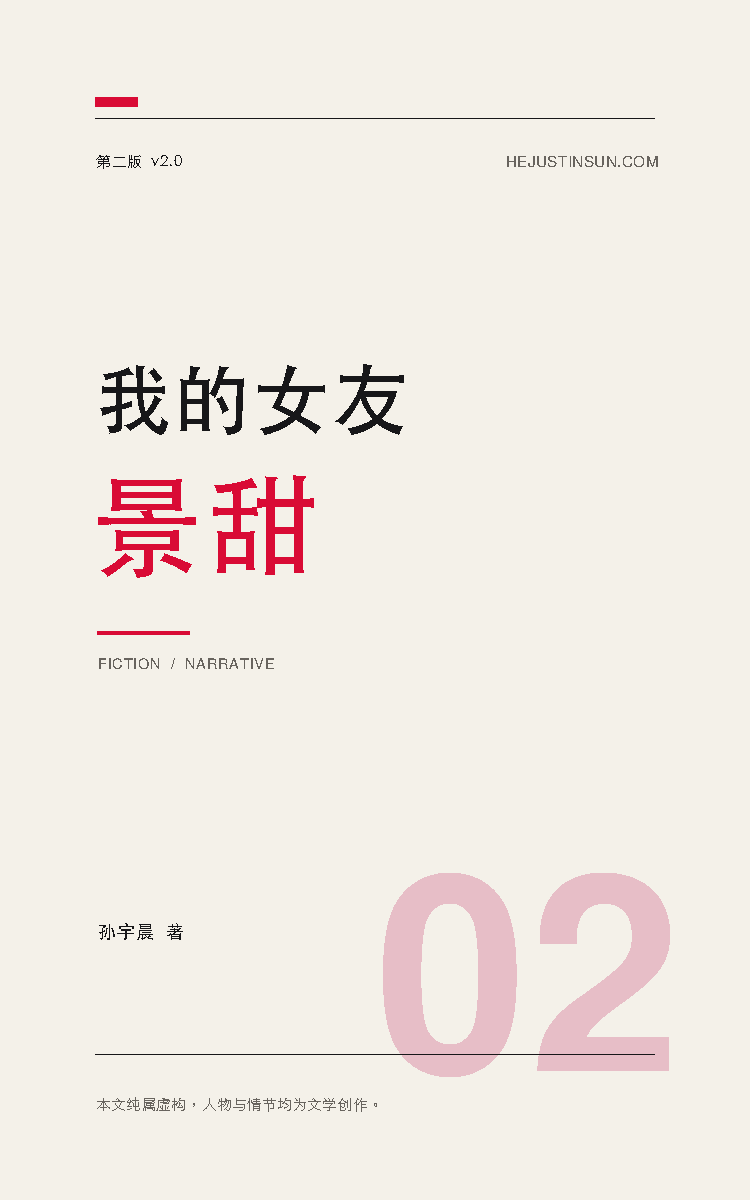
\includepdf[
  pages=1,
  fitpaper=true,
  noautoscale=true,
  pagecommand={\thispagestyle{empty}}
]{../assets/cover.pdf}

\pagenumbering{arabic}
\setcounter{page}{1}
\pagestyle{bodyrunning}
\thispagestyle{bodyopening}
% Opening-page breathing room.
\vspace*{70.817pt}

\StoryParagraph{3}{Вес одной яйцеклетки — три с половиной микрограмма.}

\StoryParagraph{3}{Вес пятидесяти миллионов долларов наличными — две с половиной тонны.}

\StoryParagraph{3}{По телефону из «Монтаж Лагуна-Бич» Цзин Тянь просила у меня второе, закладывая первое.}

\StoryParagraph{3}{Она поехала туда на пункцию яйцеклеток. Ребёнок от суррогатной матери должен был родиться в 2027 году — если поторопиться, он ещё успевал в год Лошади. Это она предложила сама. В клинике она сказала: без пятидесяти миллионов пункции не будет.}

\UnprintedPause

\StoryParagraph{0}{«Монтаж Лагуна-Бич» стоит на прибрежном обрыве, внизу — Тихий океан. Тот этаж выкупили целиком: тридцать дней, миллион долларов — ради её уединения. Она прожила восемь дней и уехала.}

\StoryParagraph{0}{Остальные двадцать два дня уборщицы отеля каждый день поднимались туда как обычно. Это рассказала моя ассистентка: сдавая ключи, она однажды застала это. Мексиканка катила тележку, заходила в номер за номером, меняла полотенца, протирала столешницы, подтыкала уголки одеял, выходила и закрывала за собой дверь. Весь этаж — два часа.}

\StoryParagraph{0}{Ассистентка спросила её: никто ведь не живёт, зачем убирать.}

\StoryParagraph{0}{Та ответила: по записям — живут.}

\StoryParagraph{0}{Версаль, потерявший королеву.}

\StoryParagraph{0}{Я вдруг понял: Цзин Тянь это нравится. Цзин Тянь нравится, когда место пустует из-за неё. Ничего не происходит.}

\StoryParagraph{3}{Вместе с «Монтаж Лагуна-Бич» пустовал и Gulfstream G700, неловко стоявший в Ван-Найсе; экипаж каждый день являлся на службу как обычно.}

\StoryParagraph{3}{На восьмой день она сделала тот звонок. После этого её больше никто не видел.}

\NarrativeBreak

\StoryParagraph{0}{В 2007 году кто-то уже жёг ради неё деньги. В тот год я только поступил в Пекинский университет.}

\StoryParagraph{3}{Жёг деньги, разумеется, не я.}

\StoryParagraph{3}{QQ выбросил всплывающее окно — в рекламе была она. На том стареньком Lenovo-IBM, разрешение мутное. Я сохранил картинку.}

\StoryParagraph{3}{Из общежития Пекинского университета, где комната стоила тысячу юаней в год, я вышел в сеть, нашёл её на Сяонэе (китайский аналог Facebook) и отправил заявку в друзья. Сяонэй требовал приписать сообщение; я писал и стирал, стирал и писал, провозился минут сорок и в конце концов отправил: «Привет».}

\StoryParagraph{3}{Она не приняла заявку.}

\StoryParagraph{3}{Возможно, она вообще не пользовалась Сяонэем.}

\StoryParagraph{3}{Все эти годы, что бы я ни делал, я думал об одном: на каком уровне она примет заявку. Я думал об этом при первом миллиарде. Думал при десяти миллиардах.}

\StoryParagraph{3}{Потом перестал. Жэньжэнь — так к тому времени назывался Сяонэй — давно закрылся.}

\StoryParagraph{3}{Второй раз я заявку не отправлял.}

\StoryParagraph{3}{В 2011 году в Пекине было холодно. Я купил пуховик за сто пятьдесят юаней. Я помню эту цену, потому что колебался три дня.}

\StoryParagraph{3}{В тот же год она снялась в фильме за сто пятьдесят миллионов — «Воюющие царства». Сунь Хунлэй, У Чжэньюй, Ким Хи Сон, Накаи Киити, Цзян У — как «Монтаж Лагуна-Бич» и Gulfstream G700 девятнадцать лет спустя — были приглашены для антуража; они не понимали, зачем они здесь, но раз уж пришли, что-то должно было случиться — но ничего не произошло.}

\StoryParagraph{3}{Потом была «Великая стена» за сто пятьдесят миллионов долларов. Чжан Имоу, Энди Лау, Мэтт Дэймон. Потом Джеки Чан. Список вселенной Цзин Тянь становился всё длиннее.}

\StoryParagraph{3}{Я к тому времени уже был в Америке — учился, строил бизнес, дел становилось всё больше. Не менялось одно: с каждой сменой устройства, как бы ни было хлопотно, я переносил ту картинку из QQ.}

\StoryParagraph{3}{Девятнадцать лет спустя в список добавили меня.}

\NarrativeBreak

\StoryParagraph{3}{В «Роузвуде» мы встретились в первый раз. Я всегда думал, что в день встречи с ней буду волноваться.}

\StoryParagraph{3}{Я не волновался.}

\StoryParagraph{3}{Она была худее, чем на фотографиях, одета просто, полулежала на диване. Я смотрел на неё и вдруг не мог вспомнить, чего же я, собственно, ждал.}

\StoryParagraph{3}{Я повёл её смотреть банан Каттелана. Она долго смотрела и спросила: сколько это стоит.}

\StoryParagraph{3}{Шесть миллионов двести тысяч долларов.}

\StoryParagraph{3}{Она сказала: а если он сгниёт?}

\StoryParagraph{3}{Я промолчал. Она сказала: ладно, пойдём лучше в кино.}

\StoryParagraph{3}{Я сказал: хорошо.}

\StoryParagraph{3}{Она сказала: в зале, кроме нас двоих, не должно быть никого.}

\StoryParagraph{3}{Я сказал: хорошо.}

\StoryParagraph{3}{Я вышел позвонить. Когда вернулся, она всё ещё стояла перед тем бананом.}

\StoryParagraph{3}{Фильм был «Зверополис 2».}

\StoryParagraph{3}{Кинозал на двоих — так обычно выглядит закрытый показ для цензоров.}

\StoryParagraph{3}{Я велел ассистенту выкупить все места в кинотеатре.}

\StoryParagraph{3}{Я читал разоблачительные статьи про накрутку кассы: билеты распроданы, а в зале сидят двое. Теперь я понял — возможно, дело не только в кассе.}

\StoryParagraph{3}{Выкупить все места несложно; сложнее с уже проданными билетами. Ассистенты и телохранители заранее встали у входа в кинотеатр и, встречая зрителей с билетами, протягивали им наличные.}

\StoryParagraph{3}{Пришла пара с ребёнком; ребёнок уже высоко держал у входа попкорн.}

\StoryParagraph{3}{Ассистент протянул пачку денег. Ребёнок не понимал, почему нельзя войти; взрослые взяли деньги, поблагодарили, ни о чём не спросили и ушли.}

\StoryParagraph{3}{В тот день деньги получили двадцать шесть человек.}

\StoryParagraph{3}{После сеанса она поменяла аватар в WeChat на офицера Джуди.}

\StoryParagraph{3}{Ночью я мял рукой её грудь, и она меня оттолкнула.}

\StoryParagraph{3}{Я решил, что она не хочет. Убрал руку и собрался что-то сказать.}

\StoryParagraph{3}{Она ничего не сказала. Села, достала из сумки маленький мешочек, расстегнула — внутри в ряд лежали какие-то штучки, похожие на крошечный набор инструментов.}

\StoryParagraph{3}{Она сказала: твои ногти царапаются, мне больно.}

\StoryParagraph{3}{Я взглянул. Я всегда стриг ногти кусачками как попало, края оставались острые — обычно этого не замечаешь.}

\StoryParagraph{3}{Она сказала: иди сюда.}

\StoryParagraph{3}{Она положила мою руку себе на колени и стала шлифовать ноготь за ногтем.}

\StoryParagraph{3}{Сначала грубой стороной, потом другой, потом ещё одной. Пошлифует немного, поднимет к лампе, посмотрит — и шлифует дальше.}

\StoryParagraph{3}{Я спросил: и долго так надо шлифовать?}

\StoryParagraph{3}{Она сказала: пока не перестанут царапаться.}

\StoryParagraph{3}{На десять пальцев у неё ушёл почти час.}

\StoryParagraph{3}{По ходу она учила меня: этой стороной — форму, этой — полировать, а последней не води туда-сюда, только в одну сторону.}

\StoryParagraph{3}{Я сказал: хорошо.}

\StoryParagraph{3}{Закончив, она повернула мою руку, посмотрела, провела пальцем.}

\StoryParagraph{3}{Она сказала: готово.}

\StoryParagraph{3}{Трогай. Где хочешь, там и трогай.}

\StoryParagraph{3}{Посреди этого она сказала одну фразу. Она сказала: если меня когда-нибудь не станет, полировать тебе ногти будет некому.}

\StoryParagraph{3}{Я усмехнулся и ничего не сказал.}

\StoryParagraph{0}{Когда мы были знакомы три месяца, я заказал одну папку. Её проекты за все годы, партнёры, доли в компаниях, Цзин Гоцин, Тянь Синьай, все связанные счета, съёмная квартира в Пекине, купленная квартира в Шанхае и кое-что ещё. Сделали за неделю, вышло сорок с лишним страниц. Были там и истории с мужчинами и женщинами — это я считал самым неважным.}

\StoryParagraph{0}{Кое-что из этого она потом рассказывала мне сама — не так, как было написано там. Я ничего не сказал.}

\StoryParagraph{0}{О чём-то она так и не рассказала. Я не спрашивал.}

\StoryParagraph{0}{Я верю всему, что она говорила.}

\StoryParagraph{0}{Ту папку я сохранил. Храню до сих пор.}

\StoryParagraph{3}{Но не верю в ней ни единому слову.}

\NarrativeBreak

\StoryParagraph{3}{Она сказала: в Гонконге слишком много людей, узнают; поедем куда-нибудь.}

\StoryParagraph{3}{Я сказал: хорошо.}

\StoryParagraph{3}{Она ткнула на карте в Тенерифе.}

\StoryParagraph{3}{Я сказал: хорошо.}

\StoryParagraph{3}{Я вышел позвонить и, только вернувшись, узнал, что это место — в Атлантике, у северо-западного берега Африки. Назавтра в полдень наша группа из тридцати человек отправилась в путь; A330 ждал в аэропорту.}

\StoryParagraph{3}{В спальне самолёта она спросила: у меня красивое имя?}

\StoryParagraph{3}{Я сказал: красивое.}

\StoryParagraph{3}{Она сказала: оно сложено из папиной фамилии и маминой — правда, удивительно?}

\StoryParagraph{3}{Я сказал: я запомнил это в первый же день.}

\StoryParagraph{3}{Она обняла меня и сказала: не зови меня больше Цзин Тянь, зови мамой.}

\StoryParagraph{3}{Хорошо, мама.}

\StoryParagraph{3}{После посадки командир подошёл и сказал: босс, остров сначала не давал посадку — они никогда не видели такого большого частного самолёта.}

\StoryParagraph{3}{На острове правила те же: вокруг не должно быть людей. Ассистенты пошли улаживать; никто не спросил зачем. В этот раз я не спросил, сколько было людей.}

\StoryParagraph{3}{«Ритц-Карлтон» стоял лицом к Атлантике, панорамные окна слишком большие. Она не может спать при малейшем свете. Ассистенты обклеили весь номер чёрной изолентой: снаружи светло как днём, внутри темно как в карцере. На солнце лента отклеивалась, каждый день переклеивали.}

\StoryParagraph{3}{Ассистентов было одиннадцать; приходили в полседьмого утра и уходили, когда мы засыпали. Ленту клеили две девушки: одна отвечала за оконные рамы, другая — за индикаторы кондиционера и розеток, после проверяли всё по три раза. Изоленты купили тридцать мотков, потом докупили ещё двадцать. Они выяснили, что наклеенная после трёх часов дня лента отваливается быстрее всего — в это время стекло горячее всего, — и стали клеить по утрам. Этому их никто не учил, они дошли сами. Они обсуждали это между собой — как обсуждают ремесло.}

\StoryParagraph{3}{Она знала, как зовут тех двух девушек. Я не знал.}

\StoryParagraph{3}{Мы остановились на обочине дороги в парке Тейде посмотреть закат; ассистенты вынесли из машины розы, открыли шампанское.}

\StoryParagraph{3}{Мама смотрела на море облаков и сказала: как красиво. Но всё же хуже, чем закат в Дэлинхе, в Цинхае.}

\StoryParagraph{3}{Я из Цинхая.}

\StoryParagraph{3}{Я не сказал этого.}

\StoryParagraph{3}{Ночью мы смотрели звёзды на вершине; даже в ватниках было холодно.}

\StoryParagraph{3}{Мама сказала: загадай желание.}

\StoryParagraph{3}{Я спросил: а ты что загадала?}

\StoryParagraph{3}{Мама сказала: не скажу.}

\StoryParagraph{3}{Мама сказала: как красиво. Только слишком холодно. Поедем на Мальдивы, а?}

\StoryParagraph{3}{Я сказал: ладно.}

\StoryParagraph{3}{На Тенерифе минус пятнадцать, на Мальдивах двадцать семь; по прямой девять с половиной тысяч километров, лететь одиннадцать часов. Только аэропорт на Мальдивах слишком мал: с нашего широкофюзеляжного пришлось бы пересесть на маленький самолёт.}

\StoryParagraph{3}{Мама сказала: маленький самолёт такой шумный. Большой лучше.}

\StoryParagraph{3}{В спальне самолёта по пути на Мальдивы мама сказала мне: её желание — ребёнок от меня. Обязательно через суррогатную мать.}

\StoryParagraph{3}{Я ни разу не спросил почему. Я думал, она боится боли.}

\StoryParagraph{3}{Посреди полёта мама вдруг села, стала искать телефон, поймала Старлинк и сказала: плохо дело.}

\StoryParagraph{3}{Я спросил: что случилось?}

\StoryParagraph{3}{Она сказала: один человек мне угрожает, три дня спрашивает, я не отвечаю.}

\StoryParagraph{3}{Я спросил: сколько нужно?}

\StoryParagraph{3}{Она сказала: не твоё дело.}

\StoryParagraph{3}{Она долго печатала: стирала и правила, правила и стирала. Напечатав, положила телефон экраном вниз на колени, потом снова перевернула и посмотрела.}

\StoryParagraph{3}{Я спросил: кто этот человек?}

\StoryParagraph{0}{Она сказала: работал со мной раньше. Финансист. Сел. Взял всё на себя.}

\StoryParagraph{3}{Вышел, деваться некуда — и обязательно надо найти меня.}

\StoryParagraph{3}{Я сказал: так сдай его полиции, и всё.}

\StoryParagraph{3}{Она взглянула на меня: ты не понимаешь.}

\StoryParagraph{3}{Я спросил: ты дала?}

\StoryParagraph{3}{Она сказала: дала.}

\StoryParagraph{3}{Сколько?}

\StoryParagraph{3}{Восемьдесят тысяч.}

\StoryParagraph{3}{Я сказал: и об этом стоило думать три дня?}

\StoryParagraph{3}{Она ничего не сказала.}

\StoryParagraph{3}{Остаток дня она почти не разговаривала. Уснула только после посадки.}

\StoryParagraph{0}{Первым в «Сонева Джани» прибыл мамин чемодан. Багаж тридцати человек в маленький самолёт не влез, разделили на три рейса. У мамы был один чемодан — отдельным рейсом: она сказала, что не хочет, чтобы он лежал рядом с чужими.}

\StoryParagraph{0}{«Сонева Джани» славится своим no news, no shoes; мама успокоилась.}

\StoryParagraph{3}{Управляющие отеля, телохранители, ассистенты — всего двадцать шесть человек, и ещё два оператора дронов держались поодаль. Ассистенты снова клеили изоленту: лампочка кондиционера, лампочки розеток, раз за разом.}

\StoryParagraph{0}{Вечером мы, как обмениваются паролями, обменялись бывшими — так династия сверяет девизы правления. Мама не хотела ни единой неточности; но у мамы было запретное слово: того спортсмена упоминать нельзя.}

\StoryParagraph{0}{Я не упомянул. Хотя знал: татуировка у мамы на спине сделана из-за спортсмена.}

\StoryParagraph{3}{Наверное, слишком большая — не сведёшь.}

\StoryParagraph{0}{Она сказала: теперь мы одна семья. Родители растили меня, это было нелегко, — ты должен дать выкуп за невесту.}

\StoryParagraph{0}{Я сказал: хорошо.}

\StoryParagraph{0}{Она назвала два имени — Цзин Гоцин, Тянь Синьай — и два счёта.}

\StoryParagraph{0}{Тридцать миллионов. Юаней.}

\StoryParagraph{0}{Я перевёл. Те два имени я впервые увидел на тех сорока с лишним страницах.}

\StoryParagraph{3}{Чуть погодя она протянула мне телефон. Тянь Синьай ответила одним словом: «Получено».}

\StoryParagraph{0}{Однажды мама сказала: знаешь, о чём я думаю, когда прошу у тебя всё это?}

\StoryParagraph{0}{Я спросил: о чём?}

\StoryParagraph{0}{Она сказала: я думаю — скажешь ли ты хоть раз «нет».}

\StoryParagraph{0}{Я сказал: не скажу.}

\StoryParagraph{0}{Она сказала: тогда неинтересно.}

\StoryParagraph{3}{А я подумал: разве есть что-то, чего я не могу?}

\StoryParagraph{0}{Когда становилось совсем скучно, я возился с той картинкой из QQ 2007 года — хотел перенести её на новое устройство. Мама сунулась посмотреть: ты что, тайком от меня хранишь фото чужой женщины? Кто это?}

\StoryParagraph{0}{Я промолчал. Ничего не сказал.}

\StoryParagraph{0}{Картинка была слишком мутная; она не разглядела и пошла заниматься другим.}

\StoryParagraph{0}{В тот вечер я удалил картинку.}

\StoryParagraph{3}{Назавтра восстановил её со старого телефона.}

\StoryParagraph{0}{Мама тоже без конца листала телефон; я спросил, что она смотрит.}

\StoryParagraph{0}{Она сказала: ничего, всё та же дрянь — борьба за первое место в титрах.}

\StoryParagraph{0}{Борьба за первое место в титрах: в картине только одна звезда может стоять первой. Даже между главным героем и главной героиней первым стоит кто-то один.}

\StoryParagraph{0}{Я сказал: какая скука.}

\StoryParagraph{0}{Она сказала: да. А ещё труднее вот что: бывают пары на съёмках — заходишь в группу на сорок-пятьдесят дней, всё время снимаешься с одним и тем же мужчиной, ночью занимаешься с ним любовью, а днём борешься за первое место в титрах.}

\StoryParagraph{0}{Я сказал: это против человеческой природы.}

\StoryParagraph{0}{Она сказала: да.}

\StoryParagraph{0}{Зато когда съёмки закончились — сколько бы раз до этого ни занимались любовью, считается, что ничего не произошло.}

\StoryParagraph{3}{Потом она листала ещё полчаса.}

\StoryParagraph{0}{2 января 2026 года, «Сонева Джани», новый год — я сделал маме предложение.}

\StoryParagraph{0}{Решил я утром 1 января. Кольцо было в Гонконге. На острове кольца не продают; ассистент улетел гидросамолётом в Мале и днём вернулся — кольцо лежало в конверте отеля.}

\StoryParagraph{0}{Мама сказала: бриллиант слишком маленький.}

\StoryParagraph{0}{Мама сказала: ничего, потом подаришь побольше.}

\StoryParagraph{0}{И ещё: ты можешь приехать в Пекин?}

\StoryParagraph{0}{Я промолчал.}

\StoryParagraph{0}{Она решила, что я не хочу ехать.}

\StoryParagraph{0}{Мама сказала: почему ты так добр ко мне?}

\StoryParagraph{0}{Я сказал: потому что ты мне нравишься.}

\StoryParagraph{0}{Она сказала: а раньше, с другими, ты тоже был таким?}

\StoryParagraph{0}{Я сказал: нет.}

\StoryParagraph{3}{Она усмехнулась и ничего не сказала.}

\StoryParagraph{0}{Однажды утром я проснулся рано — её не было в постели.}

\StoryParagraph{0}{Я вышел: она сидела на террасе лицом к морю; море было сплошь чёрное. Свет не горел, ещё не рассвело.}

\StoryParagraph{0}{Я спросил, почему она встала так рано.}

\StoryParagraph{0}{Она сказала: я считаю дни.}

\StoryParagraph{0}{Я спросил: какие дни?}

\StoryParagraph{0}{Она сказала: иди спи.}

\StoryParagraph{0}{Я посидел рядом с ней немного, не зная, что сказать. Потом пошёл спать.}

\StoryParagraph{3}{Когда я проснулся снова, она уже была накрашена.}

\StoryParagraph{0}{За четырнадцать дней на Мальдивах её не узнал ни один человек.}

\StoryParagraph{0}{Вечером тринадцатого дня в ресторане она сняла тёмные очки. Чуть погодя сняла и шляпу, положила на стол. Так она просидела весь ужин. За соседним столом — пожилая немецкая пара, официант — из Шри-Ланки; никто не взглянул на неё лишний раз.}

\StoryParagraph{0}{После ужина она снова надела шляпу.}

\StoryParagraph{0}{Мама сказала: поедем домой.}

\StoryParagraph{0}{Я сказал: мы же ещё не пожили вдоволь.}

\StoryParagraph{3}{Она сказала: слишком тихо.}

\UnprintedPause

\StoryParagraph{0}{Вернувшись в Гонконг, мама встретилась с моими родителями.}

\StoryParagraph{0}{В тот же вечер она сказала: семье надо готовить смотрины и свадьбу, одарить всех как можно щедрее. Всё те же Цзин Гоцин и Тянь Синьай.}

\StoryParagraph{0}{Я не спросил зачем.}

\StoryParagraph{0}{Я сказал: лимит одной карты — миллион в день.}

\StoryParagraph{0}{Мама сказала: слишком медленно.}

\StoryParagraph{0}{Переводи с пяти.}

\StoryParagraph{0}{Пять карт, два счёта, переводы по кругу. На третьей карте я на мгновение заколебался. Но перевёл всё.}

\StoryParagraph{3}{Мама сказала: слишком низкая эффективность.}

\StoryParagraph{0}{Я сказал: давай на Новый год привезём наших родителей в Гонконг и встретим вместе.}

\StoryParagraph{0}{Мама сказала: в этом году уже решено встречать на Хайнане. В следующем.}

\StoryParagraph{0}{В праздник над гаванью Виктория пускали фейерверк, пришёл миллион человек. Её не было.}

\StoryParagraph{0}{В три часа ночи я отвёз родителей домой.}

\StoryParagraph{0}{Дорога была пустая; на красном не ждала ни одна машина — я всё равно остановился.}

\StoryParagraph{0}{Мама сказала: пока не будем видеться — скоро лететь в Лос-Анджелес на пункцию. Сначала надо закончить дела.}

\StoryParagraph{0}{Мама снова спросила: ты можешь приехать в Пекин?}

\StoryParagraph{0}{Я промолчал.}

\StoryParagraph{3}{Она не сказала, что в Пекине. Я не спросил.}

\StoryParagraph{0}{Мама сказала: в Гонконге обязательно нужно купить квартиру — на её имя.}

\StoryParagraph{0}{Я сказал: ладно.}

\StoryParagraph{3}{На День святого Валентина мы тоже не увиделись.}

\StoryParagraph{0}{Однажды по телефону она сказала: сегодня утром взяли восемь пробирок крови.}

\StoryParagraph{0}{Я сказал: так много.}

\StoryParagraph{0}{Она сказала: ничего.}

\StoryParagraph{0}{Я сказал: досталось тебе.}

\StoryParagraph{0}{Потом мы говорили о другом.}

\StoryParagraph{0}{Только позже я узнал: такую кровь сдают натощак, на второй или третий день цикла, день перепутать нельзя. В то утро она вышла из дома, наверное, часов в шесть; пекинская зима, ещё темно. Обследований потом становилось всё больше. Я знал об этом, потому что в ежемесячной сводке платежей у ассистента появилась новая строка. Впервые — в прошлом году, сумма небольшая, несколько тысяч. Потом каждый месяц, иногда по два-три платежа. Я утверждал их быстро. Такие суммы не требуют смотреть расшифровку. Лишь потом я узнал, что это были анализы крови, панель из шести гормонов, УЗИ, АМГ. Смотрели, какой у неё остался резерв, сколько удастся взять, стоит ли идти дальше.}

\StoryParagraph{0}{Всё это делалось в Пекине.}

\StoryParagraph{3}{Я не знаю, в какой больнице. Не знаю и того, ездила она одна или с кем-то.}

\StoryParagraph{0}{25 февраля она приземлилась в Гонконге.}

\StoryParagraph{0}{Она сказала: в Лос-Анджелес не поедет, пока не увидит квартиру в Гонконге.}

\StoryParagraph{0}{Я переслал ей всю подборку за полгода — десяток с лишним квартир. Все ей показались некрасивыми. Ни в одной из них я не был; ассистент полгода отбирал их одну за другой, ассистент пересылал мне, я — ей. Одна была в Мид-Лэвелс — в видео виднелась гавань Виктория, снимали в сумерках. На миг камера дрогнула и поймала на стене тень человека, который снимал. Я смотрел на эту тень и думал: кто он, сколько он сегодня прошёл, сколько квартир посмотрел, знает ли он, для кого эта квартира.}

\StoryParagraph{3}{Времени было в обрез; она всё-таки села на G700 до Лос-Анджелеса и 28 февраля прилетела в «Монтаж Лагуна-Бич».}

\NarrativeBreak

\StoryParagraph{0}{На восьмой день мама позвонила. У неё был день, у меня — глубокая ночь.}

\StoryParagraph{0}{Она сказала: пятьдесят миллионов. Долларов.}

\StoryParagraph{0}{Я сказал: дай подумать.}

\StoryParagraph{0}{Она молчала. Я слышал, что у неё там море.}

\StoryParagraph{0}{Помолчав, она сказала: хорошо.}

\StoryParagraph{0}{Она повесила трубку.}

\StoryParagraph{3}{За всё время, что я её знал, я ни разу не говорил ей «дай подумать».}

\StoryParagraph{0}{В Claude Code я через API прогнал все свои денежные активы; вывод: на меня это никак не повлияет. Я сверил ещё раз. Я ввёл вопрос в Claude Code. Claude сказал: не отдавай ей эти пятьдесят миллионов долларов.}

\StoryParagraph{3}{Я спросил: она меня больше не любит?}

\StoryParagraph{3}{Claude сказал: любовь меня не занимает, и я её не понимаю. Но эти пятьдесят миллионов долларов ты ей отдать не должен.}

\StoryParagraph{3}{Я никогда ей не отказывал — не из щедрости, из страха. Из страха перед ответом в следующую секунду.}

\StoryParagraph{0}{А теперь кто-то сказал это за меня.}

\StoryParagraph{0}{Я долго смотрел на эту строку. Мороз по коже у меня пошёл не от того, что он умён, а от того, что Claude ни секунды не колебался.}

\StoryParagraph{0}{Ему не трудно.}

\StoryParagraph{0}{Я тогда подумал: наверное, это что-то высшее. Человек так не может.}

\StoryParagraph{3}{Она меня больше не любит?}

\StoryParagraph{3}{На следующий день она перезвонила.}

\StoryParagraph{3}{Мама сказала: море большое.}

\StoryParagraph{3}{Я сказал: да?}

\StoryParagraph{3}{Она сказала: этаж слишком большой, эхо. Утром приходят убирать — я прячусь в ванной и жду, пока они уйдут.}

\StoryParagraph{3}{Я сказал: можно, чтобы они не приходили.}

\StoryParagraph{3}{Она сказала: не надо.}

\StoryParagraph{3}{Она сказала: в клинике спрашивают, когда приедет отец ребёнка.}

\StoryParagraph{3}{Я сказал: я могу прислать людей.}

\StoryParagraph{3}{Она сказала: не надо.}

\StoryParagraph{3}{Потом она сказала: ты подумал?}

\StoryParagraph{3}{Я молчал. Не потому что думал — я не думал ни о чём. В трубке у неё там было море, у меня — гавань Виктория, и с обеих сторон никто не говорил ни слова. Я посчитал: одиннадцать секунд.}

\StoryParagraph{3}{Цзин Тянь сказала: ладно.}

\StoryParagraph{3}{Цзин Тянь сказала: я поняла.}

\StoryParagraph{3}{Она повесила трубку.}

\StoryParagraph{3}{Потом я бессчётное число раз вспоминал: что ещё она говорила в те два дня, кроме пятидесяти миллионов. Море большое. Этаж слишком большой. Она прячется в ванной. Вот и всё — я помню всё, слово в слово. Чего я не могу вспомнить — её голос: каким тоном она сказала «я поняла».}

\StoryParagraph{0}{Не могу вспомнить. Потом я перестал вспоминать.}

\StoryParagraph{0}{Я положил телефон на тумбочку экраном вниз. Потом я сделал одну вещь, до сих пор не знаю зачем: положил руку на грудь и посчитал.}

\StoryParagraph{0}{Сердце билось ровно.}

\StoryParagraph{0}{Я посчитал ещё раз — по-прежнему ровно. Шестьдесят с чем-то в минуту, как всегда. Я сидел, прижав руку к собственной груди, как врач, осматривающий кого-то другого.}

\StoryParagraph{3}{Я подумал: вот, значит, как.}

\StoryParagraph{0}{Остаток дня я не делал ничего. Я просидел в номере, пока не стемнело и снова не рассвело, глядя, как гавань Виктория из синей становится серой, потом чёрной. В шесть утра в финансовом центре напротив, здание за зданием, начали зажигаться огни. Один раз постучал ассистент, спросил, что с ужином; я сказал: не нужно.}

\StoryParagraph{3}{Я не плакал. Я всё ждал, когда заплачу.}

\NarrativeBreak

\StoryParagraph{0}{Потом ассистент сводил со мной счета; там была и компенсация отелю на Тенерифе. После нашего отъезда ленту клеили ещё несколько дней — никто не сказал девушкам, что больше не нужно. Отель заявил: клеили слишком долго и слишком много раз, следы клея с рам не оттираются, стекло придётся менять целиком.}

\StoryParagraph{0}{Я сказал: утверждаю.}

\StoryParagraph{3}{То стекло смотрит на Атлантику.}

\StoryParagraph{0}{Строка топлива в счёте вышла дороже, чем тот этаж в «Монтаже». Я поинтересовался. Ассистент сказал: A330 рассчитан на двести человек, нас тридцать, самолёт слишком лёгкий, центровка на взлёте не сходится. Поэтому каждый раз доливают лишнее топливо — до нужного веса. А по прилёте лишнее оставлять нельзя, его сливают.}

\StoryParagraph{0}{Я спросил: каждый раз так?}

\StoryParagraph{3}{Он сказал: каждый раз так.}

\StoryParagraph{0}{Ещё была коробка, присланная из лос-анджелесской клиники. Уколы для стимуляции на восемь дней, хранить в холоде, ни один не вскрыт.}

\StoryParagraph{3}{Ещё задаток агентству суррогатного материнства, двести тысяч долларов, не возвращается. Женщину нашли ещё в январе: калифорнийка, тридцать четыре года, рожала дважды. В досье есть её фотография; я не смотрел. Она была готова ещё в январе.}

\StoryParagraph{3}{После ухода Цзин Тянь я ещё раз достал ту фотографию 2007 года. Девятнадцать лет; пиксели в устройствах всё выше, а у этой картинки разрешение словно всё ниже — лицо размыто. Я долго вглядывался, увеличив её: искал, чем она отличалась от той, какой стала потом. Не нашёл ни одного отличия. Потому что на той картинке с самого начала ничего не разглядеть.}

\StoryParagraph{0}{Однажды я стриг ногти кусачками; постриг, провёл пальцем — острые.}

\StoryParagraph{0}{Я вспомнил: в ящике ещё лежит та штука, которую она оставила.}

\StoryParagraph{0}{Я достал, шлифанул пару раз — не то. Она говорила: только в одну сторону. Я забыл, в какую.}

\StoryParagraph{0}{Я положил её обратно.}

\StoryParagraph{3}{Мои ногти до сих пор царапаются.}

\StoryParagraph{0}{Однажды утром на телефоне всплыло напоминание — ассистент поставил его в прошлом году, составляя календарь: за три месяца до родов подготовить комнату.}

\StoryParagraph{3}{Я смахнул его.}

\StoryParagraph{0}{После её ухода я всё думаю об одном.}

\StoryParagraph{0}{Если бы в тот день я дал — она бы осталась?}

\StoryParagraph{0}{Я думал очень долго.}

\StoryParagraph{3}{Потом я достал ту папку и перечитал ещё раз. Сорок с лишним страниц.}

\StoryParagraph{0}{А потом я вспомнил вечер праздника — как с крыши смотрел на фейерверк над гаванью Виктория.}

\StoryParagraph{0}{Миллион человек прихлынул, как прилив; фейерверк кончился — миллион человек отхлынул.}

\StoryParagraph{0}{Миллион человек.}

\StoryParagraph{0}{Так каждый год.}

\StoryParagraph{0}{Гонконг, три часа ночи —}

\StoryParagraph{3}{Ничего не произошло.}

\end{document}
